\chapter{Выполнение}

\section{Выбор языка программирования}

Для выполнения домашнего задания был выбран язык C++.

\section{Код программы}

В листинге 2.1 представлен код программы.

\begin{lstlisting}[caption=Алгоритм исправления орфографических ошибок в тексте]
	void single_thread(const string &input_text, const vector<string> &dictionary)
	{
		string temp_text = input_text; // 1
		istringstream iss(temp_text); // 2
		vector<string> words(istream_iterator<string>{iss}, istream_iterator<string>{}); // 3
		for (auto &word : words) // 4
		{
			int min_distance = numeric_limits<int>::max(); // 5
			string best_match = word; // 6
			
			for (auto &dict_word : dictionary) // 7
			{
				int distance = alg_lev(word, dict_word); // 8
				
				if (distance < min_distance) // 9
				{
					min_distance = distance; // 10
					best_match = dict_word; // 11
				}
			}
			size_t pos = temp_text.find(word); // 12
			
			while (pos != string::npos) // 13
			{
				temp_text.replace(pos, word.length(), best_match); // 14
				pos = temp_text.find(word, pos + best_match.length()); // 15
			}
		}
	}
\end{lstlisting}

\section{Графовые модели программы}

\subsection{Граф управления}

На рисунке~\ref{fig:control_graph} представлен граф управления.

\begin{figure}[h!]
	\centering{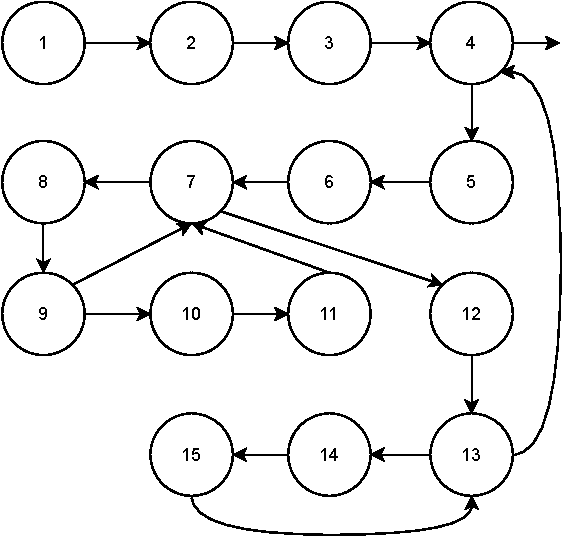
\includegraphics[scale=1]{photos/control_graph.pdf}}
	\caption{Граф управления}
	\label{fig:control_graph}
\end{figure}

\clearpage

\subsection{Информационный граф}

На рисунке~\ref{fig:info_graph} представлен информационный граф.

\begin{figure}[h!]
	\centering{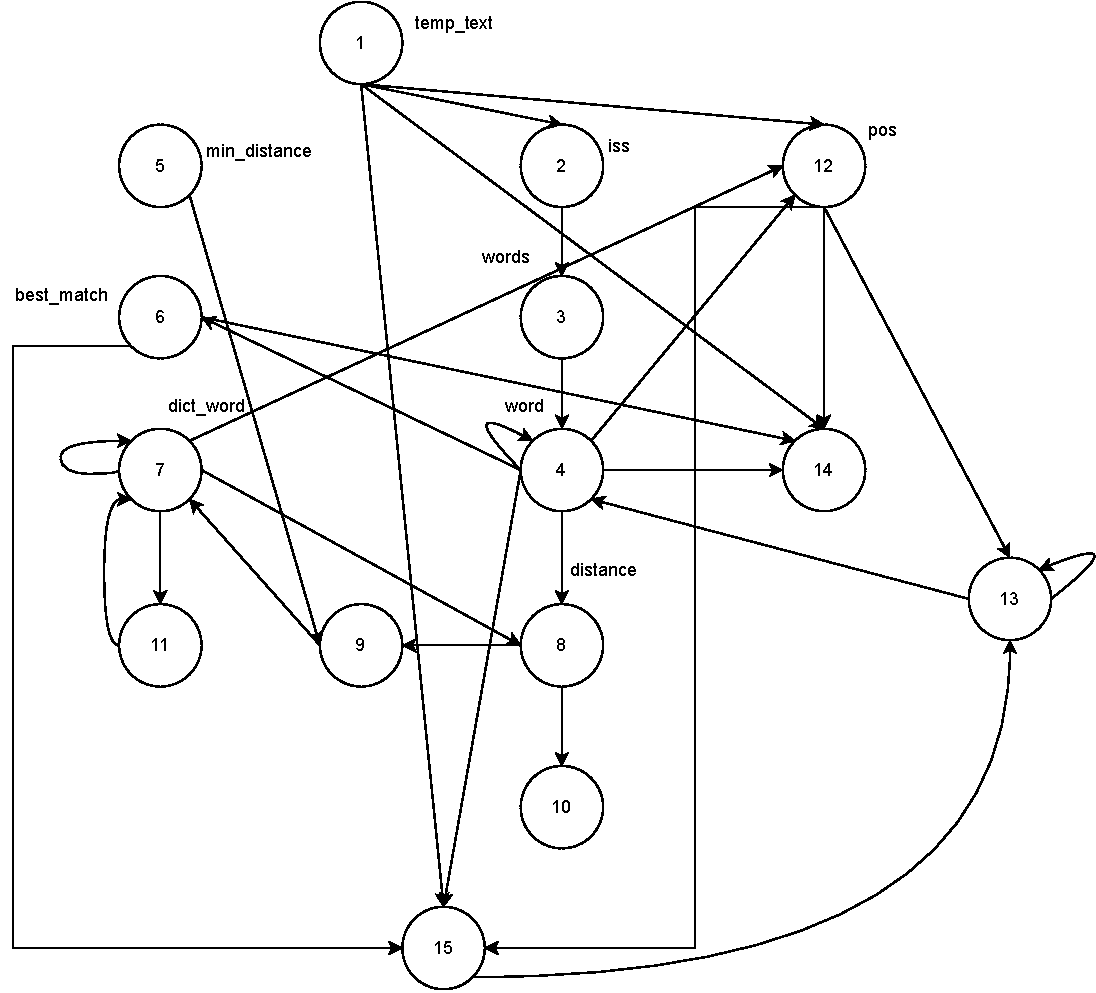
\includegraphics[scale=0.9]{photos/info_graph.pdf}}
	\caption{Информационный граф}
	\label{fig:info_graph}
\end{figure}

\clearpage

\subsection{Операционная история}

Дан следующий короткий текст «hellw rorld».

На русунке~\ref{fig:oper_history} представленна операционная история.

\begin{figure}[h!]
	\centering{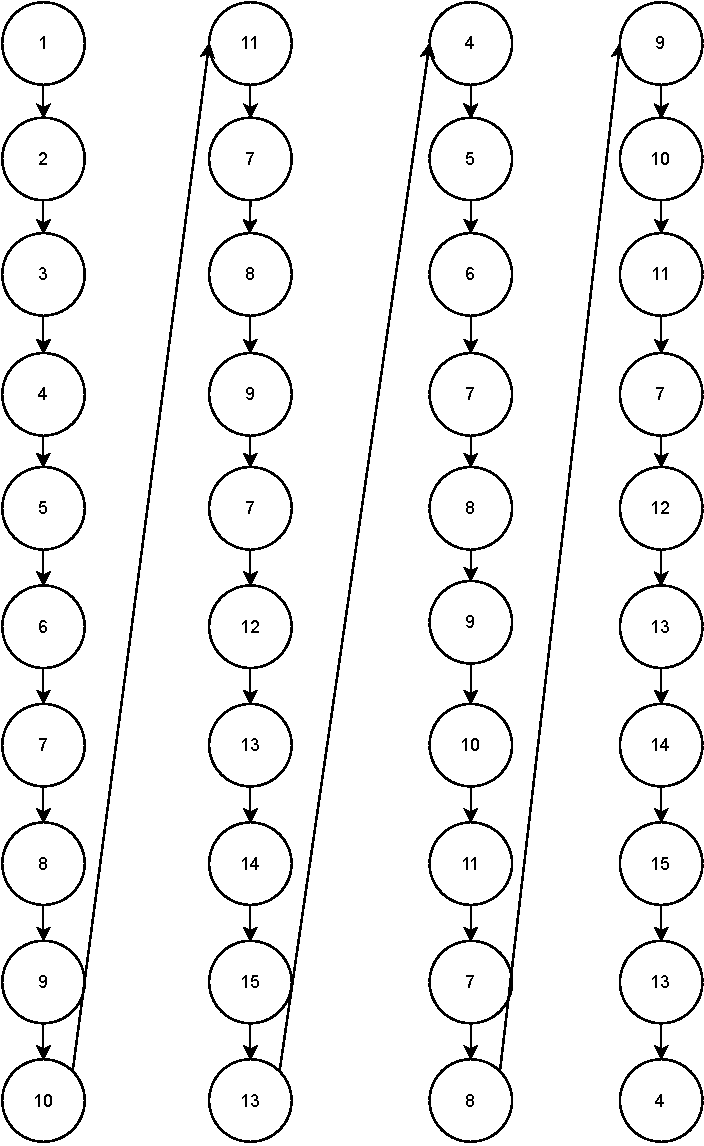
\includegraphics[scale=0.9]{photos/oper_history.pdf}}
	\caption{Операционная история}
	\label{fig:oper_history}
\end{figure}

\clearpage

\subsection{Информационная история}

На рисунке~\ref{fig:info_history} представленна информационная история.

\begin{figure}[h!]
	\centering{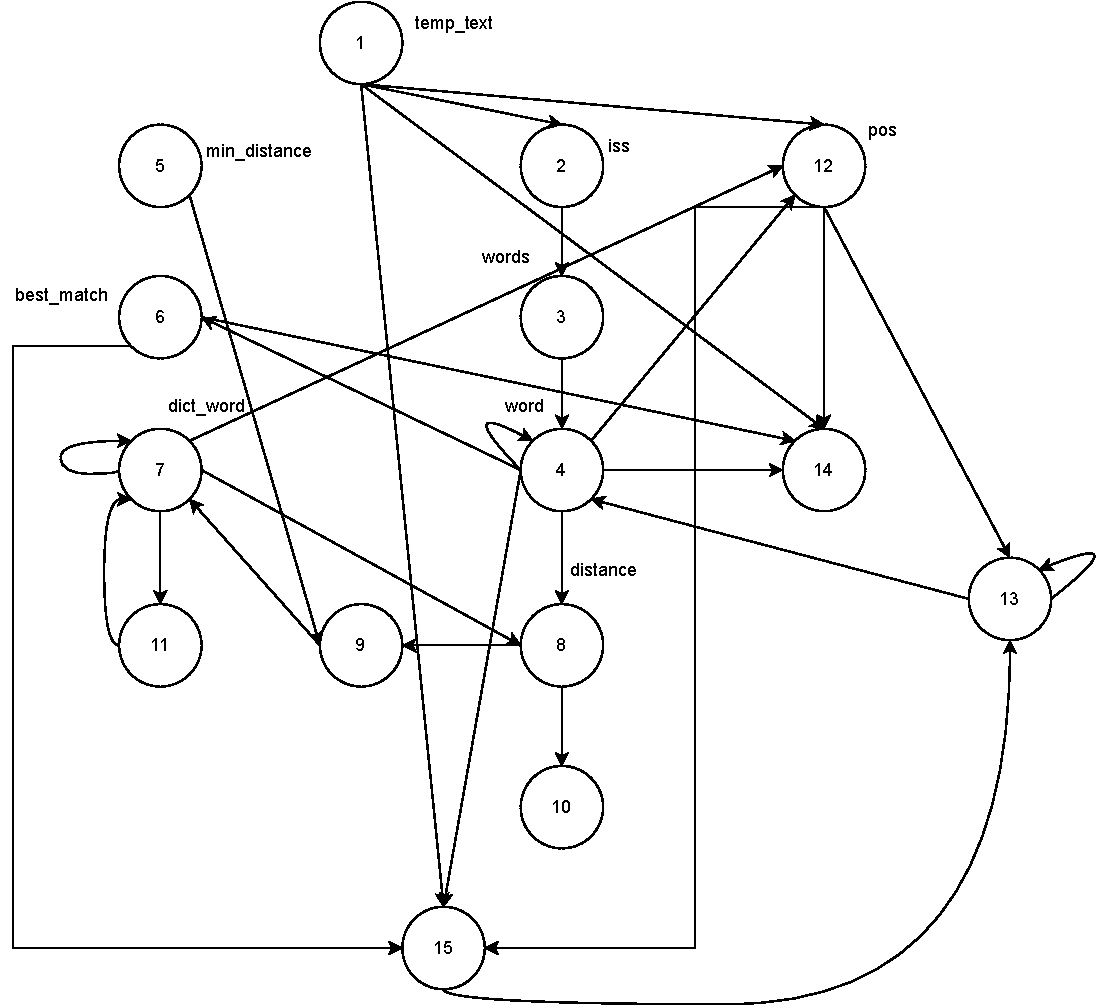
\includegraphics[scale=0.9]{photos/info_history.pdf}}
	\caption{Информационная история}
	\label{fig:info_history}
\end{figure}




